\documentclass{beamer}
 
\usepackage[utf8]{inputenc}
\usepackage{mystyle}
\usepackage{magic_dice}

%Information to be included in the title page:
\title{DiCE: The Infinitely Differentiable Monte Carlo Estimator}
\author{Anonymous}
\institute{Overleaf}
\date{2014}
 
\newcommand{\dice}{{\scshape DiCE}} 
\newcommand{\magicbox}{{\scshape MagicBox}} 
 
\begin{document}
 
\frame{\titlepage}
 
\begin{frame}
\frametitle{Motivation}
\begin{itemize}
\item The score function estimator is widely used for estimating gradients of
objectives involving stochastic computation graphs, i.e. objectives that look like $\Es{x}{f(x)}$
\item Convenient to define a \textit{surrogate loss} (SL)
whose derivative is the gradient estimator for use in auto-diff (Schulman et al., 2015) 
\item However, recursive application of the surrogate loss procedure leads to incorrect
higher order derivatives
\item DiCE provides a simple and correct programmatic recipe for doing so
\end{itemize}
\end{frame}

\begin{frame}
\frametitle{Notation}
\begin{itemize}
\item Random variables $x$
\item All functions parameterized by and all gradients taken wrt $\theta$
\item Will drop $\theta$ subscripts after a while
\item The $\bot(\cdot)$ operator sets the gradient to zero (.detach)
\end{itemize}
\end{frame}

\begin{frame}
\frametitle{Surrogate Loss (SL)}
\begin{itemize}
\item Loss of interest 
$$\mcL(\theta) = \Es{p_\theta(x)}{f_\theta(x)}$$
\item Surrogate loss
$$SL(f, \theta, x) = \bot(f_\theta(x))\log p_\theta(x) + f_\theta(x)$$
\item Where the gradient of the surrogate loss is an unbiased estimator of the gradient of 
the original loss
$$\nabla_\theta \mcL(\theta) = \Es{p_\theta(x)}{\nabla_\theta SL(f, \theta, x)}$$
\item SL scales the log prob of the actions $x$
using the detached cost $\bot(f(x))$ 
\end{itemize}
\end{frame}

\begin{frame}
\frametitle{First derivative}
\begin{itemize}
\item The gradient of the original loss is given by
\begin{align*}
\nabla_\theta \mcL(\theta)
&= \Es{x}{\mathbin{\color{red}{f_\theta(x)}}\nabla_\theta \log p_\theta(x) + \nabla_\theta f_\theta(x)}\\
&=\Es{x}{g(x)}
\end{align*}
\item The gradient of the surrogate loss is given by
\begin{align*}
\nabla_\theta SL(f, \theta, x)
&= \nabla_\theta \bot(f_\theta(x))\log p_\theta(x) + \nabla_\theta f_\theta(x)\\
&= \mathbin{\color{red}{\bot(f_\theta(x))}}
    \nabla_\theta \log p_\theta(x) + \nabla_\theta f_\theta(x)\\
&= g_{SL}(x)
\end{align*}
where the extra term $\log p_\theta(x) \nabla_\theta f_\theta(x)$ 
would be included if not for the $\bot(\cdot)$ operator
\item The gradient-stoppage of $\mathbin{\color{red}{\bot(f_\theta(x))}}$ in $g_{SL}(x)$
will cause issues with higher order gradients
\end{itemize}
\end{frame}

\begin{frame}
\frametitle{Second derivative}
\begin{itemize}
\item Second derivative of original loss
\begin{align*}
\nabla^2_\theta \mcL(\theta) &= \nabla_\theta\Es{x}{g(x)}\\
&= \Es{x}{g(x)\nabla_\theta\log p_\theta(x) + \mathbin{\color{red}{\nabla_\theta g(x)}}}
\end{align*}
\item Recursive application of SL to $g_{SL}(x)$
\begin{align*}
SL(g_{SL}, \theta, x) &= \log p_\theta(x)\bot(g_{SL}(x)) + g_{SL}(x)\\
\E{\nabla_\theta SL(g_{SL}, \theta, x)}
&= \E{\bot(g_{SL}(x))\nabla_\theta\log p_\theta(x) + \mathbin{\color{red}{\nabla_\theta g_{SL}(x)}}}
\end{align*}
\item However, $\nabla_\theta g(x) \neq \nabla_\theta g_{SL}(x)$
(but $g(x) = g_{SL}(x)$)
because of the stopped-gradient term in $g_{SL}$
\end{itemize}
\end{frame}

\begin{frame}
\frametitle{Missing term}
\begin{itemize}
\item We have
\begin{align*}
\nabla g(x) &= \nabla f(x)\nabla \log p(x)                              &+ f(x)\nabla^2\log p(x)       &+ \nabla^2 f(x)\\
\nabla g_{SL}(x) &= \underbrace{\nabla \bot(f(x))\nabla \log p(x)}_{=0} &+ \bot(f(x))\nabla^2\log p(x) &+ \nabla^2 f(x)
\end{align*}
\end{itemize}
\end{frame}

\begin{frame}
\frametitle{Summary}
\begin{itemize}
\item SL works if you apply it a single time
\item SL fails if you try to apply it recursively,
since the gradient truncation $\bot(\cdot)$
drops dependencies
\item This means there is no way to use SL programmatically
to obtain higher-order gradient estimators
\item \dice{} gives us a way to use autodiff to obtain higher-order gradients
\end{itemize}
\end{frame}
 
\begin{frame}
\frametitle{\dice{} and \magicbox{} $(\magic)$}
\begin{itemize}
\item Introduce the \magicbox{} operator with the following properties
\begin{enumerate}
\item $\magic(x) \rightarrowtail$ 1
\item $\nabla_\theta\magic(x) = \magic(x)\nabla_\theta \log p_\theta(x)$
\end{enumerate}
\item Intuition
\begin{enumerate}
\item Does not change evaluation, so we can apply this directly to the original objective
\item Serves the same purpose as SL but recovers dropped dependency
\end{enumerate}
\end{itemize}
\end{frame}
 
\begin{frame}
\frametitle{A nicer loss}
\begin{itemize}
\item Introduce the \dice{} objective
$$\mcL_{\magic} = \magic(x)f(x)$$
with
\begin{align*}
\magic(x) &= \exp(\tau - \bot(\tau))\\
\tau &= \log p(x)
\end{align*}
\end{itemize}
\end{frame}
 
\begin{frame}
\frametitle{Cost-centric}
\begin{itemize}
\item The \dice{} objective is cost-centric
\item We augment the objective at every cost node
\end{itemize}
\vspace{2em}
\centering
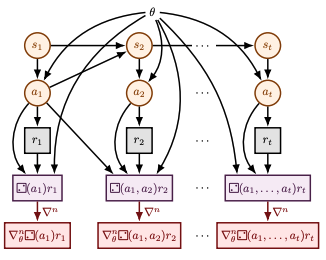
\includegraphics[height=1in]{dicegraph.png}
\end{frame}
 
\begin{frame}
\frametitle{Cost-centric}
\begin{itemize}
\item Whereas SL is action-centric
\item SL augments the objective at every stochastic node
\end{itemize}
\vspace{2em}
\centering
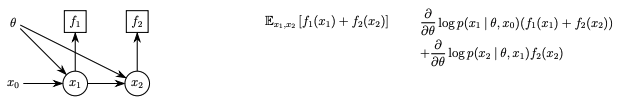
\includegraphics[height=0.75in]{slgraph.png}
\end{frame}
 

\end{document}
